\pdfminorversion=4
\documentclass[aspectratio=169]{beamer}

\mode<presentation>
{
  \usetheme{default}
  \usecolortheme{default}
  \usefonttheme{default}
  \setbeamertemplate{navigation symbols}{}
  \setbeamertemplate{caption}[numbered]
  \setbeamertemplate{footline}[frame number]  % or "page number"
  \setbeamercolor{frametitle}{fg=white}
  \setbeamercolor{footline}{fg=black}
} 

\usepackage[english]{babel}
\usepackage[utf8x]{inputenc}
\usepackage{tikz}
\usepackage{courier}
\usepackage{array}
\usepackage{bold-extra}
\usepackage{minted}
\usepackage[thicklines]{cancel}
\usepackage{ulem}
\usepackage{fancyvrb}

\xdefinecolor{dianablue}{rgb}{0.18,0.24,0.31}
\xdefinecolor{darkblue}{rgb}{0.1,0.1,0.7}
\xdefinecolor{darkgreen}{rgb}{0,0.5,0}
\xdefinecolor{darkgrey}{rgb}{0.35,0.35,0.35}
\xdefinecolor{darkorange}{rgb}{0.8,0.5,0}
\xdefinecolor{darkred}{rgb}{0.7,0,0}
\definecolor{darkgreen}{rgb}{0,0.6,0}
\definecolor{mauve}{rgb}{0.58,0,0.82}

\title[2021-12-06-uvirginia-hep-languages]{Programming Languages, Toolkits, and Communities \\ in Particle Physics Data Analysis}
\author{Jim Pivarski}
\institute{Princeton University -- IRIS-HEP}
\date{December 6, 2021}

\usetikzlibrary{shapes.callouts}

\begin{document}

\logo{\pgfputat{\pgfxy(0.11, 7.4)}{\pgfbox[right,base]{\tikz{\filldraw[fill=dianablue, draw=none] (0 cm, 0 cm) rectangle (50 cm, 1 cm);}\mbox{\hspace{-8 cm}
\includegraphics[height=1 cm]{princeton-logo-long.png}\hspace{0.1 cm}\raisebox{0.1 cm}{
\includegraphics[height=0.8 cm]{iris-hep-logo-long.png}}\hspace{0.1 cm}}}}}

\begin{frame}
  \titlepage
\end{frame}

\logo{\pgfputat{\pgfxy(0.11, 7.4)}{\pgfbox[right,base]{\tikz{\filldraw[fill=dianablue, draw=none] (0 cm, 0 cm) rectangle (50 cm, 1 cm);}\mbox{\hspace{-8 cm}
\includegraphics[height=1 cm]{princeton-logo.png}\hspace{0.1 cm}\raisebox{0.1 cm}{
\includegraphics[height=0.8 cm]{iris-hep-logo.png}}\hspace{0.1 cm}}}}}

% Uncomment these lines for an automatically generated outline.
%\begin{frame}{Outline}
%  \tableofcontents
%\end{frame}

% START START START START START START START START START START START START START

\begin{frame}{Very rough outline of this talk}
\vspace{0.15 cm}
\begin{columns}
\column{1.15\linewidth}
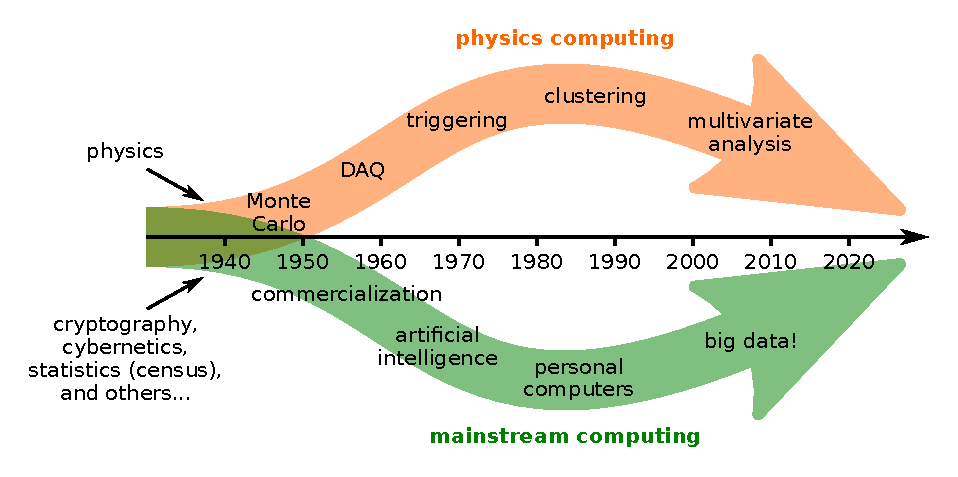
\includegraphics[width=\linewidth]{PLOTS/grand-timeline.pdf}
\end{columns}
\end{frame}

\begin{frame}{Fun fact!}
\Large
\begin{center}
\only<2>{\vspace{-0.3 cm}}
\textcolor{darkblue}{\only<1>{Did you know physicists invented the first digital computer?}\only<2>{Did you know \xcancel{physicists invented the first digital computer}?}\only<3>{Did you know physicists invented \textcolor{purple}{one of} the first digital computers?}}
\end{center}
\end{frame}

\begin{frame}{Not these\ldots}
\vspace{0.5 cm}

\begin{columns}
\column{0.5\linewidth}
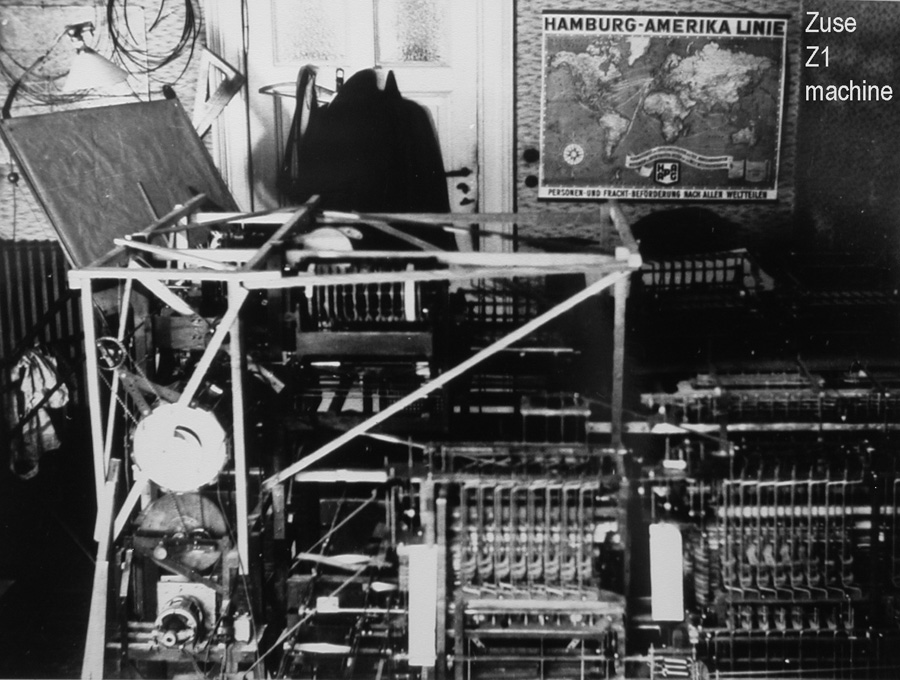
\includegraphics[width=\linewidth]{PLOTS/zuse-z1-living-room.jpg}
\column{0.5\linewidth}
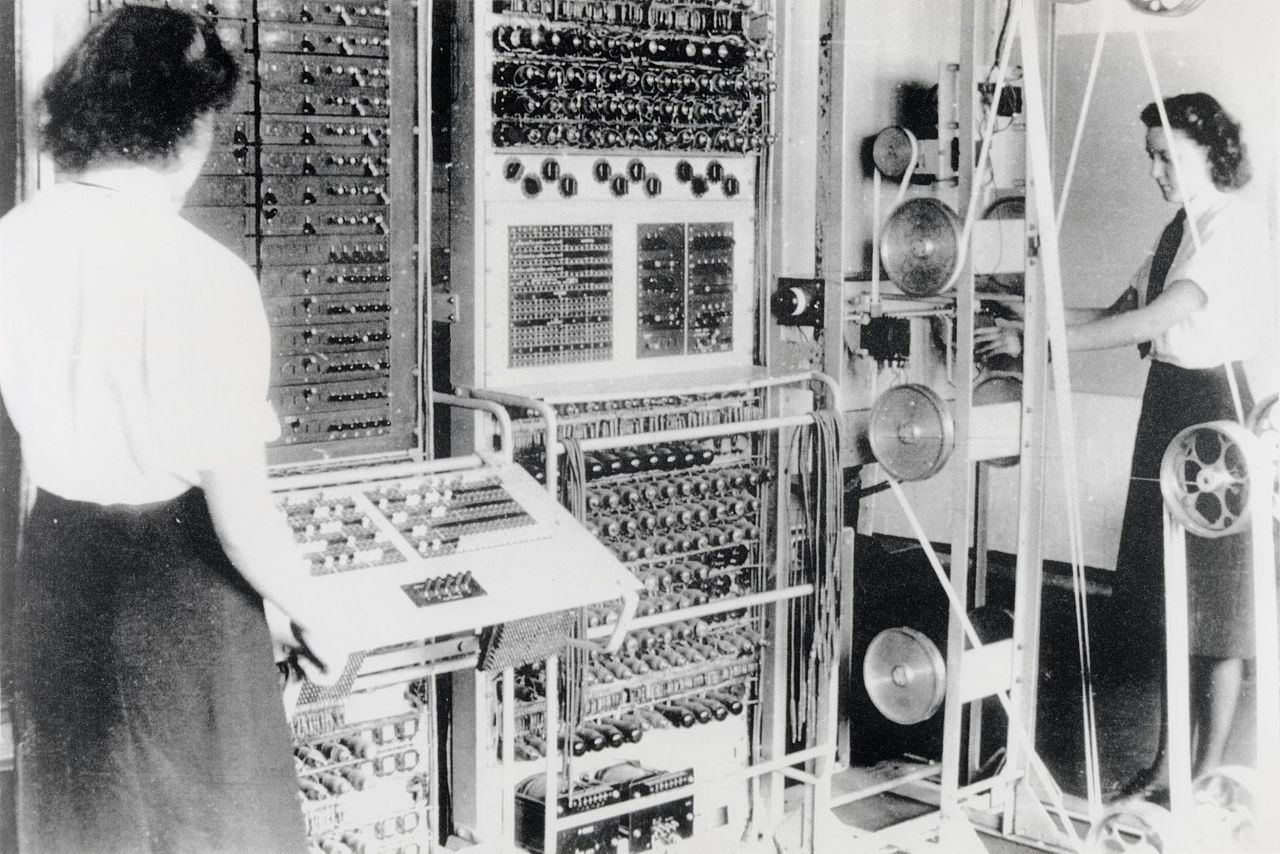
\includegraphics[width=\linewidth]{PLOTS/dorothy-du-boisson-AND-elsie-booker-COLOSSUS-MARK2.jpg}
\end{columns}

\vspace{0.5 cm}
\begin{columns}[t]
\column{0.5\linewidth}
Konrad Zuse's Z1 computer, built in his parents' living room in Berlin in 1937 (destroyed with all blueprints in 1943).

\column{0.5\linewidth}
Colossus Mark 2, operated here by Dorothy Du Boisson and Elsie Booker at Britain's secret codebreaking lab in 1943.
\end{columns}
\end{frame}

\begin{frame}{This one: ENIAC, the first {\it widely-known} digital computer (1945)}
\vspace{0.35 cm}

\mbox{\hspace{-0.25 cm}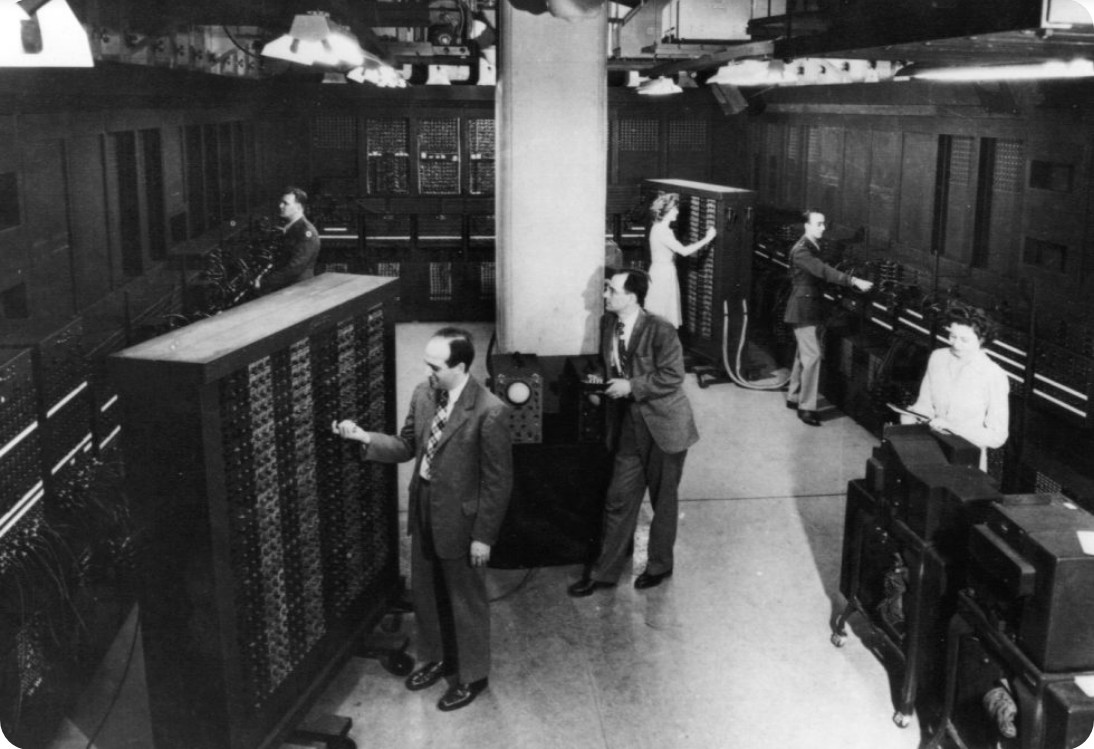
\includegraphics[height=7.5 cm]{PLOTS/eniac-1.jpg}}

\begin{onlyenv}<2->
\vspace{-7.5 cm}
\mbox{\hspace{0.75 cm}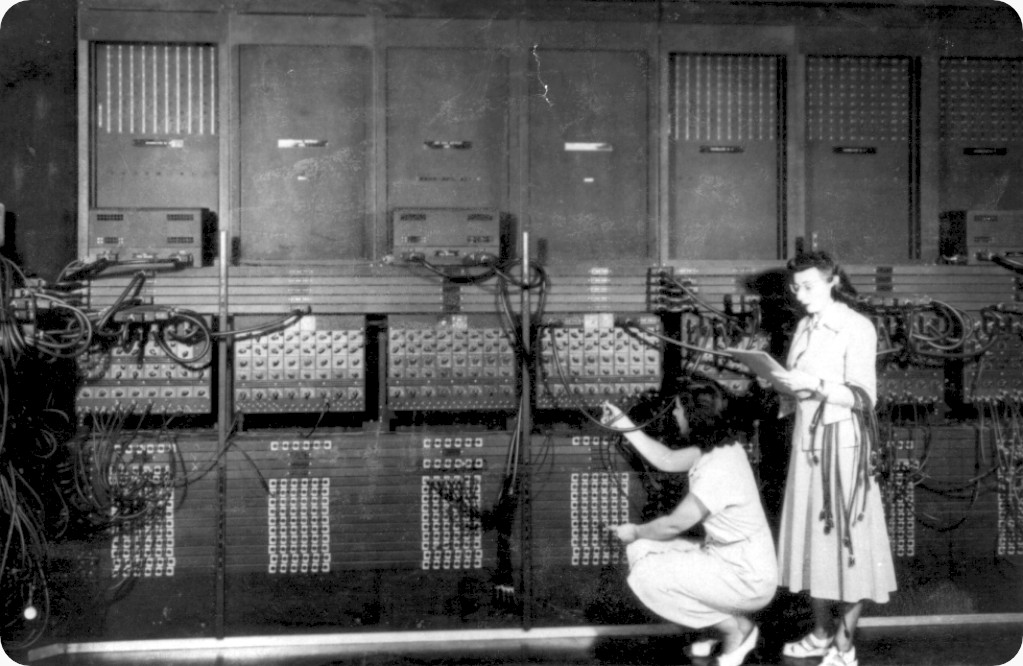
\includegraphics[height=7.5 cm]{PLOTS/eniac-2.jpg}}
\end{onlyenv}

\begin{onlyenv}<3->
\vspace{-7.5 cm}
\mbox{\hspace{1.75 cm}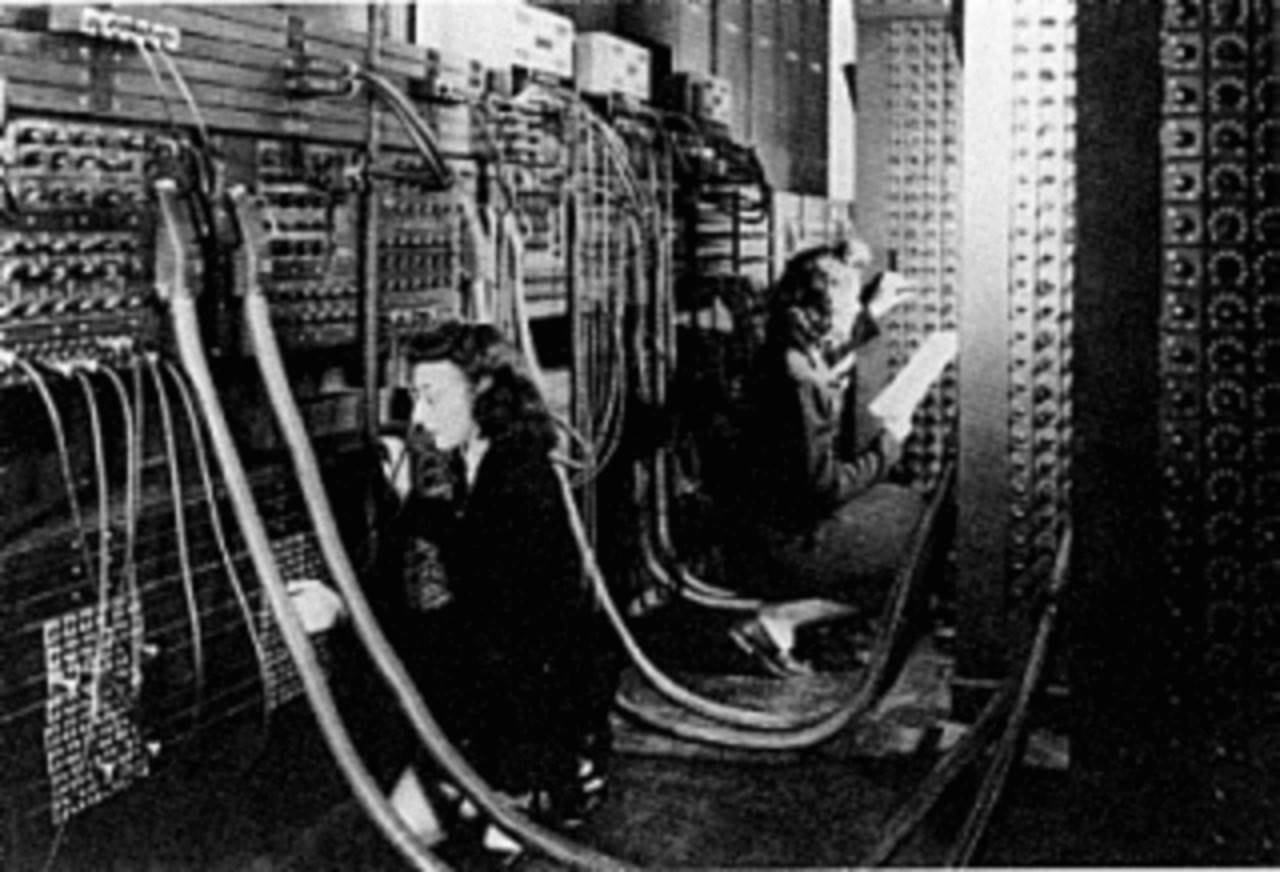
\includegraphics[height=7.5 cm]{PLOTS/eniac-3.jpg}}
\end{onlyenv}

\begin{onlyenv}<4->
\vspace{-7.5 cm}
\mbox{\hspace{2.75 cm}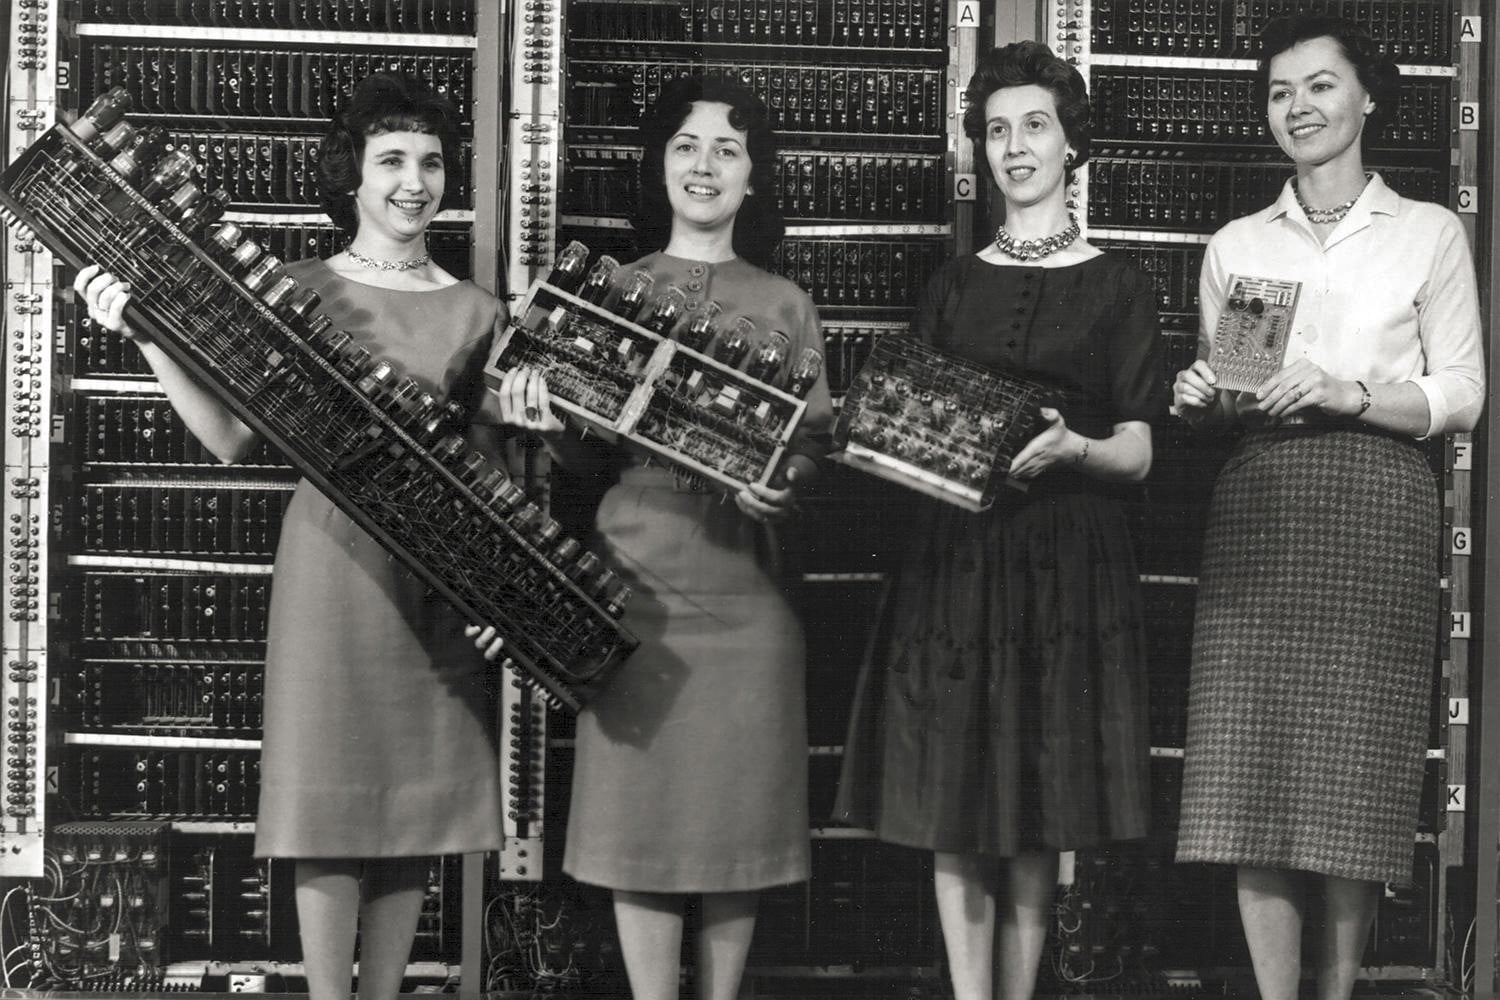
\includegraphics[height=7.5 cm]{PLOTS/eniac-4.jpg}}
\end{onlyenv}
\end{frame}

\begin{frame}{Hardware designed by}
\vspace{0.15 cm}
\begin{center}
J.\ Presper Eckert, electrical engineer, and John Mauchly, physicist (at U.\ Pennsylvania)

\vspace{0.25 cm}
\mbox{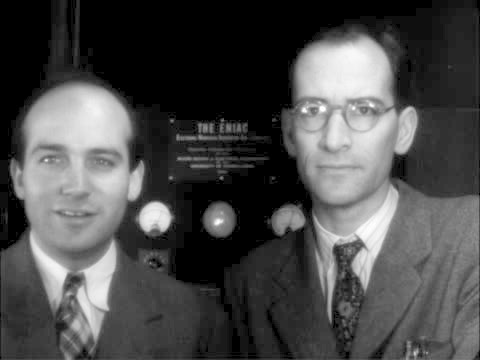
\includegraphics[height=5 cm]{PLOTS/john-mauchly-AND-presper-eckert.jpg}\only<2>{\hspace{0.1 cm}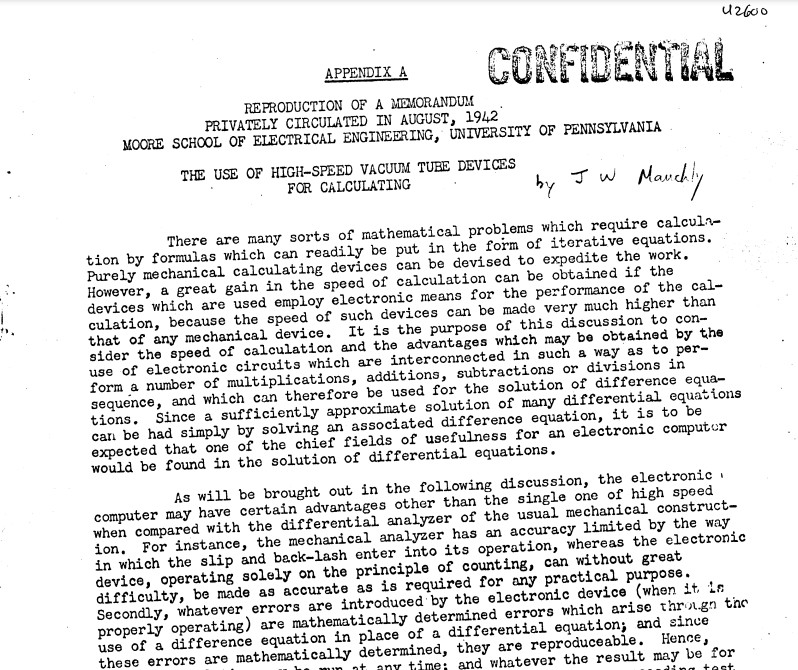
\includegraphics[height=5 cm]{PLOTS/mauchly-report.jpg}}\only<3>{\hspace{0.1 cm}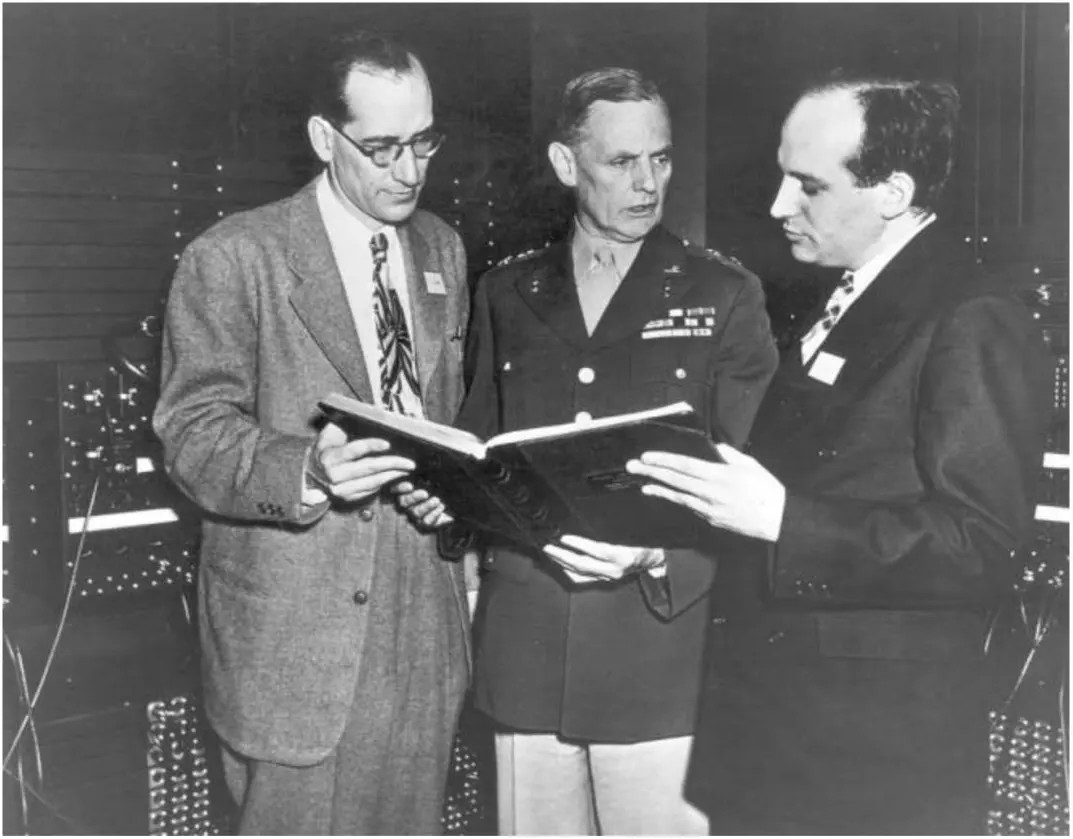
\includegraphics[height=5 cm]{PLOTS/mauchly-eckert-AND-gladeon-barnes.jpg}}}
\end{center}

\uncover<2->{Mauchly proposed ``The Use of High-Speed Vacuum Tube Devices for Calculating.''}

\vspace{0.1 cm}
\uncover<3->{It was funded (project led by Army General Gladeon Barnes) and computed artillery trajectories 1000$\times$ faster than mechanical computers, 2400$\times$ faster than humans.}
\end{frame}

\begin{frame}{John von Neumann recognized its significance}
\vspace{0.15 cm}
\begin{center}
\mbox{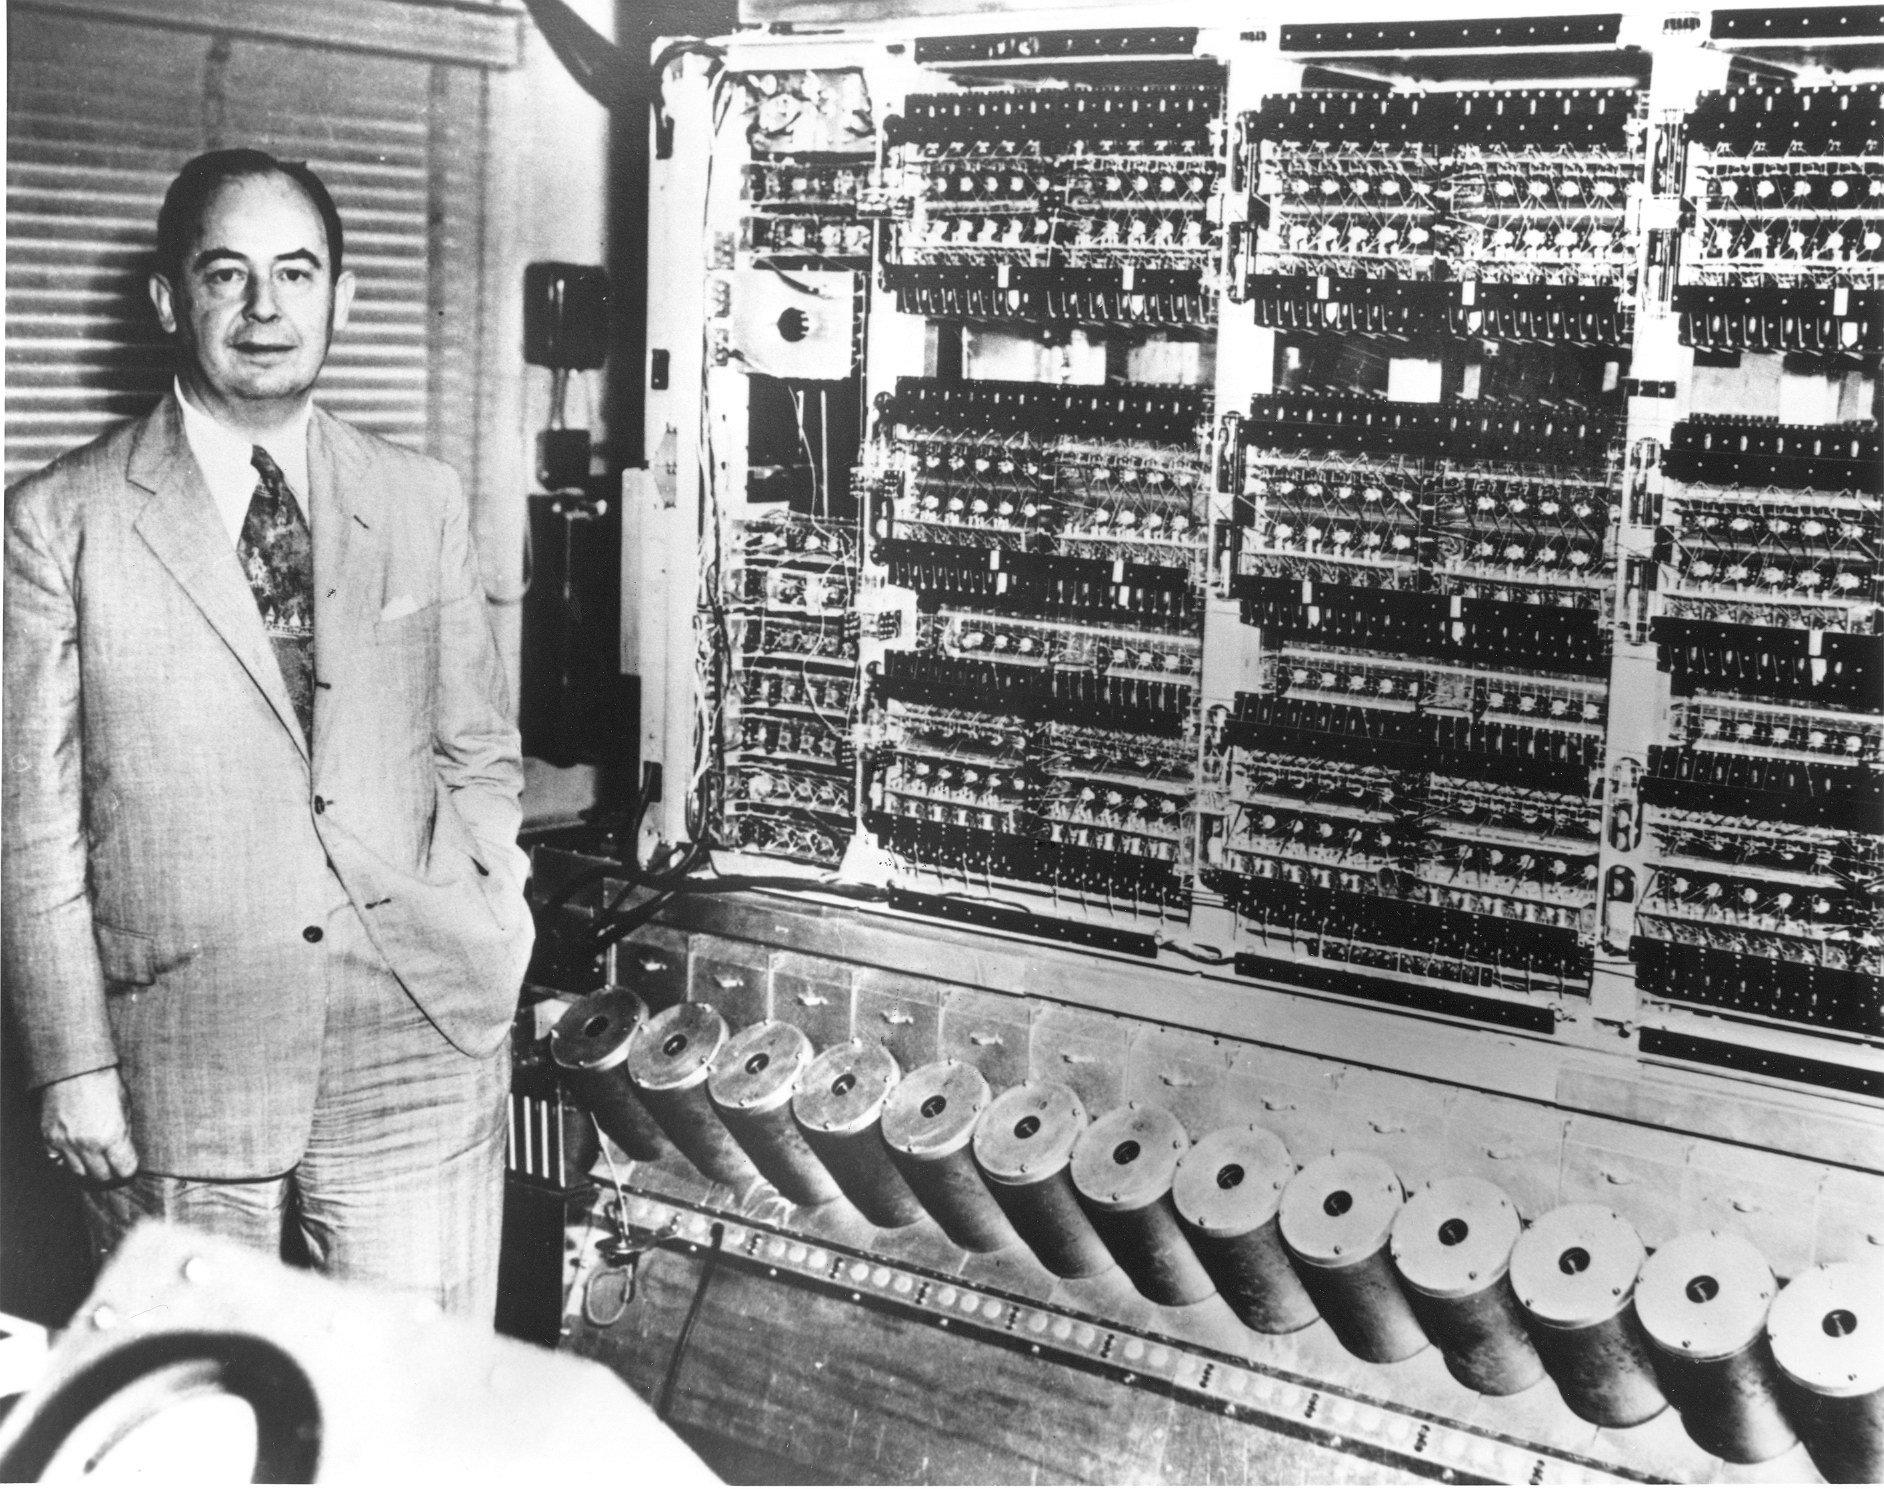
\includegraphics[height=5 cm]{PLOTS/von-neumann-edvac.jpg}\only<2>{\hspace{0.4 cm}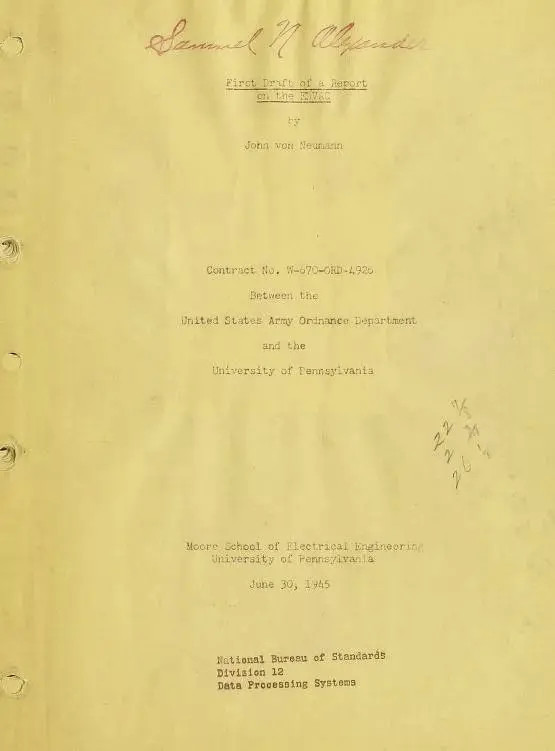
\includegraphics[height=5 cm]{PLOTS/von-neumann-architecture.jpg}}}
\end{center}

He saw that it could be reprogrammed to compute neutron diffusion for the Manhattan Project, using Stanislaw Ulam's random-number method, codenamed ``Monte Carlo.''

\vspace{0.1 cm}
\uncover<2->{While consulting for Mauchly and Eckert's second computer, EDVAC (pictured above), he described its novel stored-program design in a single-author report, which is why it's now called the ``von Neumann architecture.''}
\end{frame}

\begin{frame}{FERMIAC}
\begin{columns}
\column{1.05\linewidth}
\begin{center}
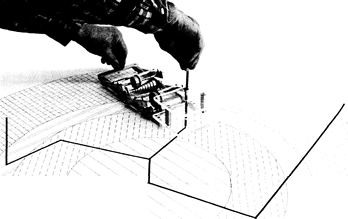
\includegraphics[height=5.5 cm]{PLOTS/FERMIAC.jpg}\hspace{0.25 cm}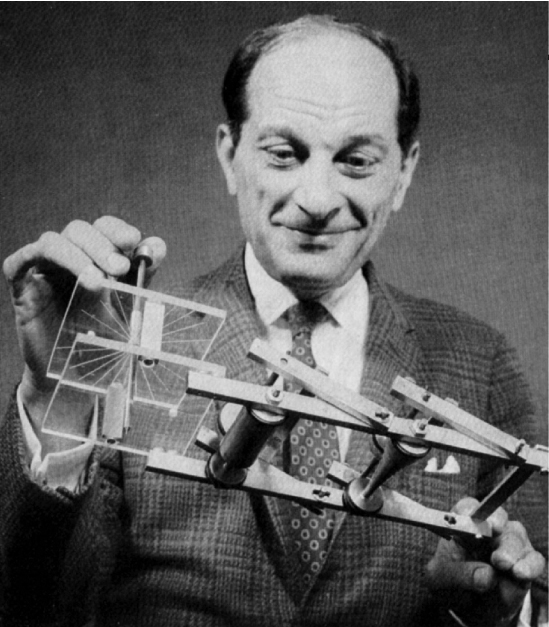
\includegraphics[height=5.5 cm]{PLOTS/STAN_ULAM_HOLDING_THE_FERMIAC.jpg}
\end{center}

While waiting for the computer to be shipped, Enrico Fermi invented an analog device to perform Monte Carlo calculations by hand. (Right: Stanislaw Ulam and the FERMIAC.)
\end{columns}
\end{frame}

\begin{frame}{MANIAC (Los Alamos, 1952)}
\large
\begin{center}
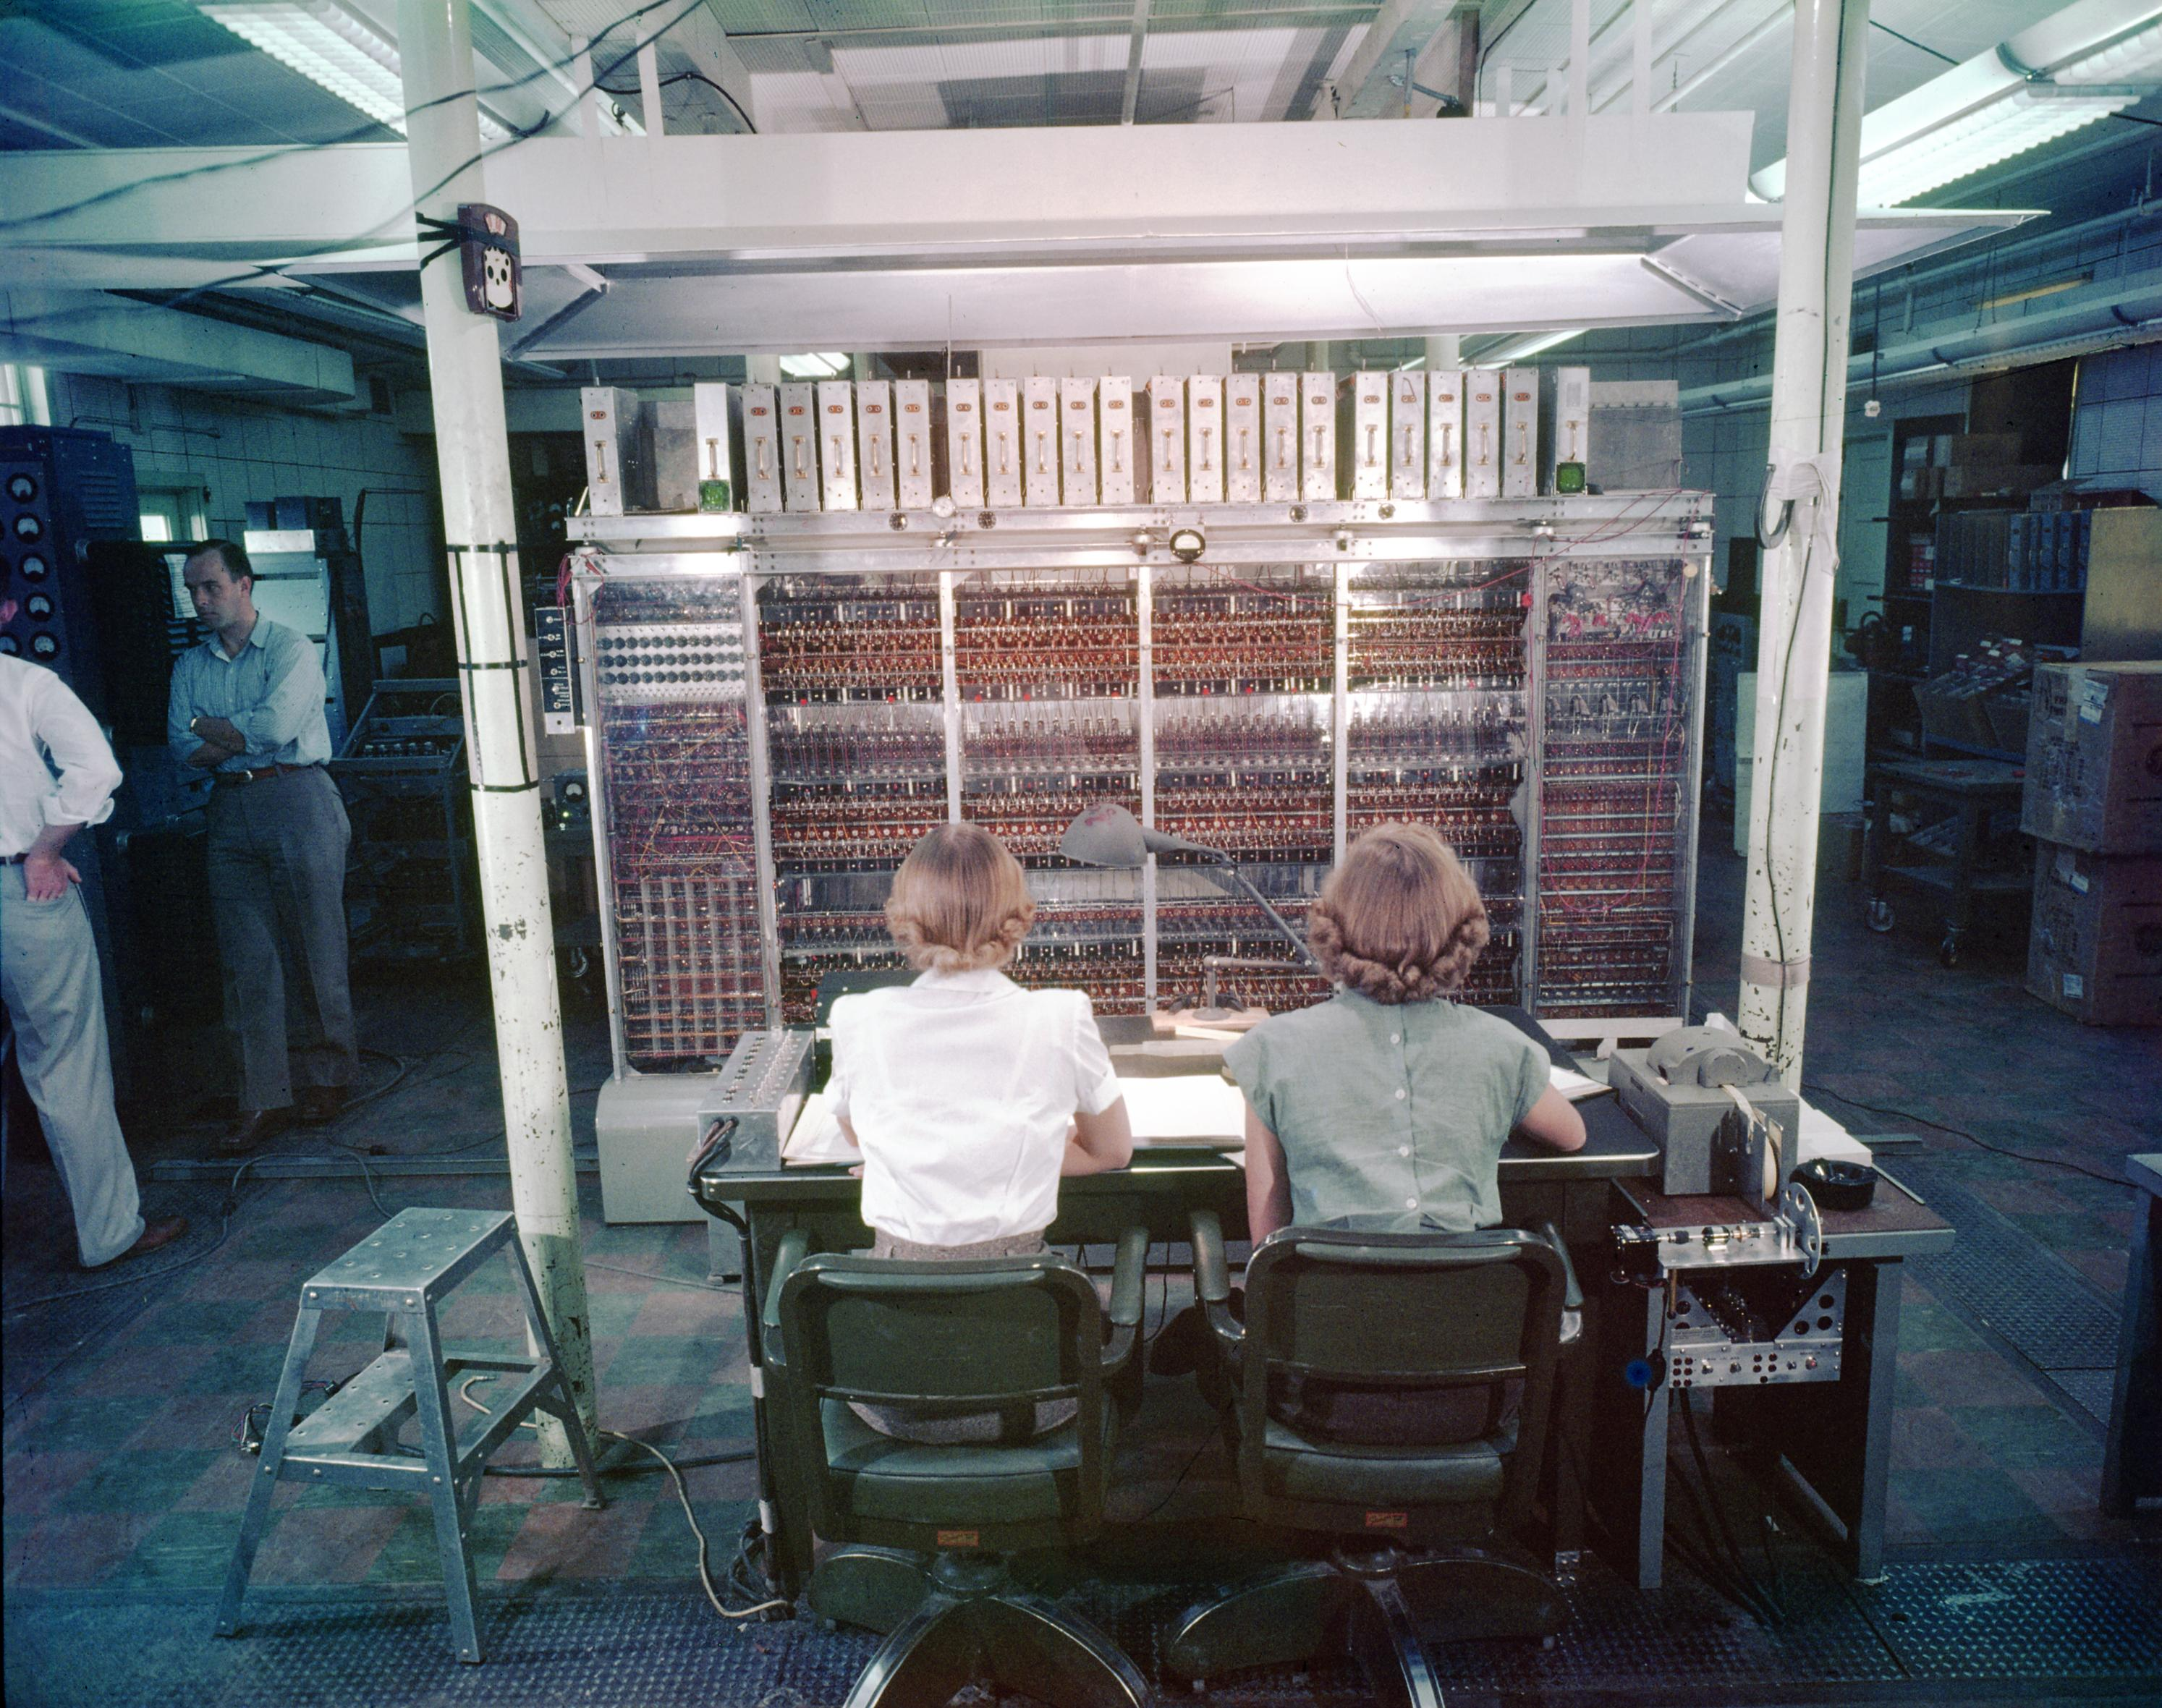
\includegraphics[height=5 cm]{PLOTS/1952-Maniac-1.jpg}\hspace{0.1 cm}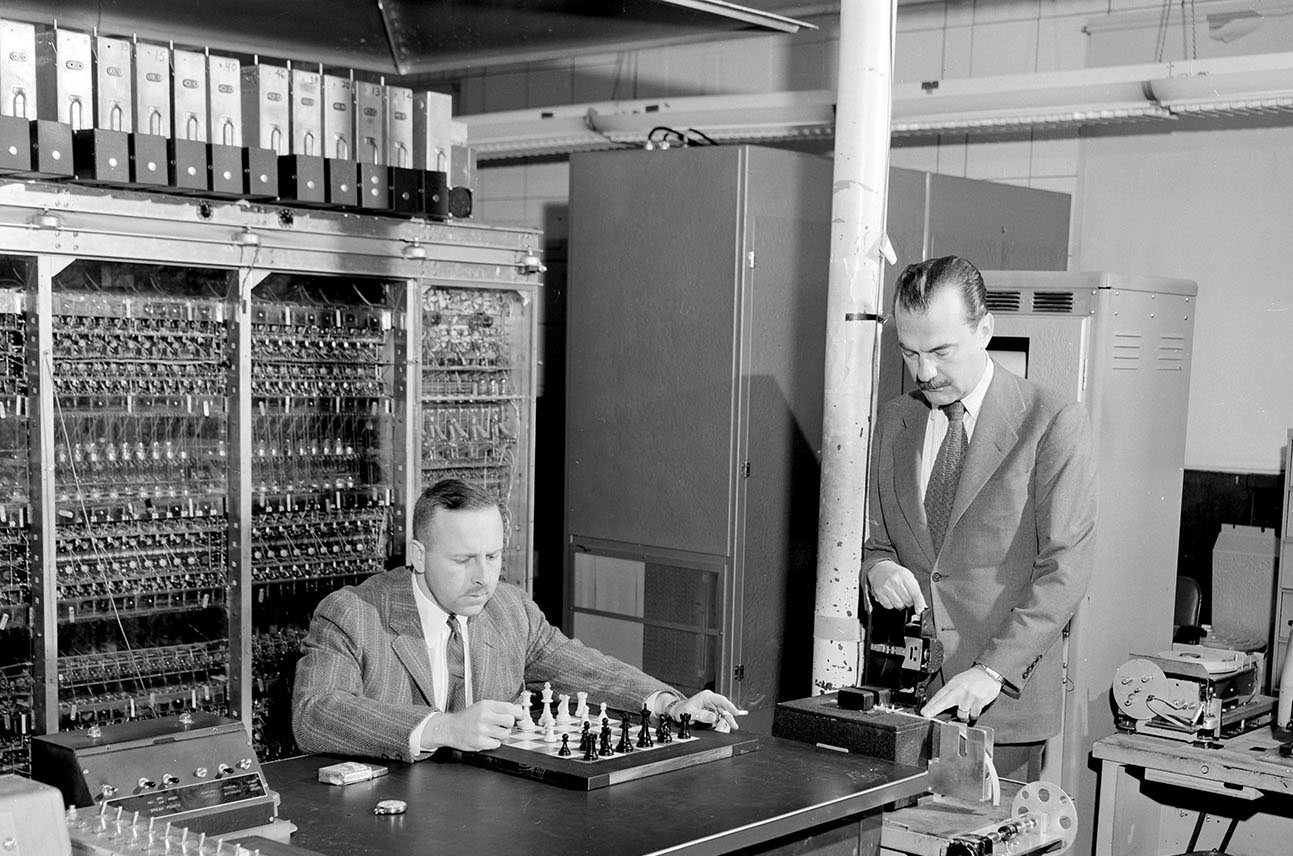
\includegraphics[height=5 cm]{PLOTS/metropolis.jpg}

\newcommand\redsout{\bgroup\markoverwith{\textcolor{red}{\rule[0.5ex]{2pt}{0.8pt}}}\ULon}

\vspace{0.5 cm}
\only<1>{{\bf M}athematical {\bf A}nalyzer {\bf N}umerical {\bf I}ntegrator and {\bf A}utomatic {\bf C}omputer}\only<2>{\redsout{{\bf M}athematical {\bf A}nalyzer {\bf N}umerical {\bf I}ntegrator and {\bf A}utomatic {\bf C}omputer}}\only<3>{{\bf M}etropolis {\bf A}nd {\bf N}eumann {\bf I}nvent {\bf A}wful {\bf C}ontraption}
\end{center}
\end{frame}

\begin{frame}{Meanwhile, Mauchly and Eckert went into industry}

\begin{center}
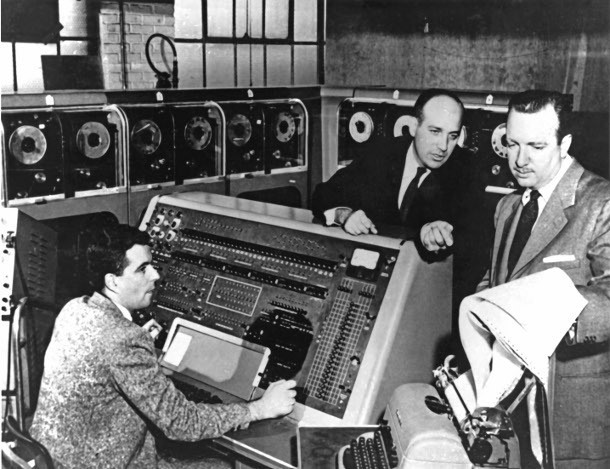
\includegraphics[height=5.5 cm]{PLOTS/univac-walter-cronkite.jpg}\only<3>{\hspace{0.3 cm}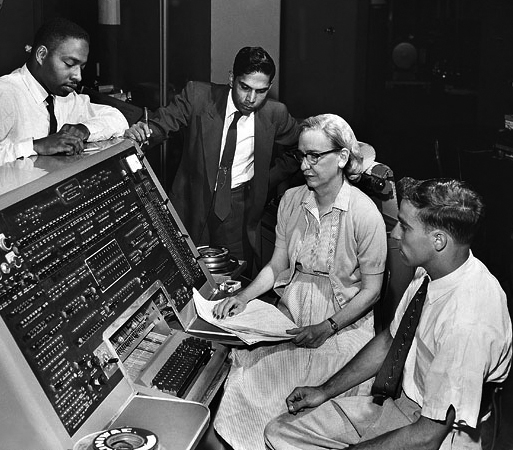
\includegraphics[height=5.5 cm]{PLOTS/Grace_Hopper_and_UNIVAC.jpg}}
\end{center}

Eckert–Mauchly Computer Corporation produced UNIVAC systems for clients.

\vspace{0.1 cm}
\uncover<2->{As a promotion, they had it predict the 1952 presidential election on live TV. It predicted Eisenhower in a landslide (with only 5\% of the votes), contrary to polls.}
\end{frame}

\begin{frame}{Programming languages}
\vspace{0.35 cm}
\begin{itemize}\setlength{\itemsep}{0.35 cm}
\item<1-> ENIAC (1945) was programmed by ``plugboard,'' wiring up a sequence of steps.

\item<2-> EDVAC (1949) stored instructions in memory as series of integers: machine code.

\item<3-> Kathleen Booth's assembly language (1947): still a series of instructions, but transliterated to a readable notation (technical design for ARC in Manchester).

\vspace{0.1 cm}
\begin{columns}
\column{0.75\linewidth}
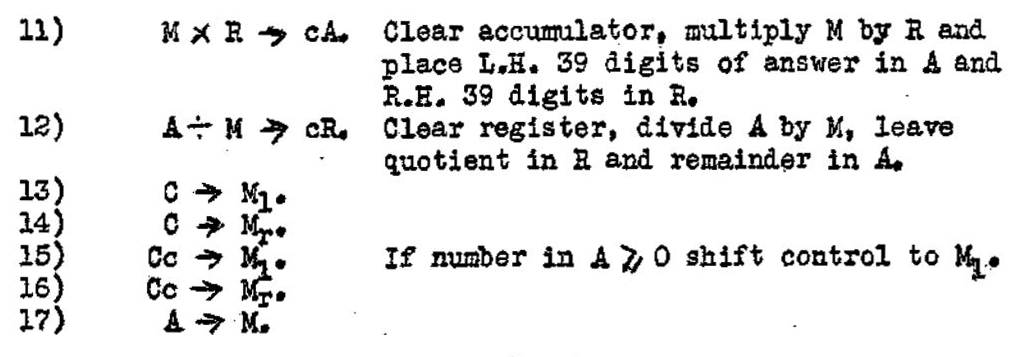
\includegraphics[width=\linewidth]{PLOTS/contracted-notation-kathleen-booth.png}

\column{0.25\linewidth}
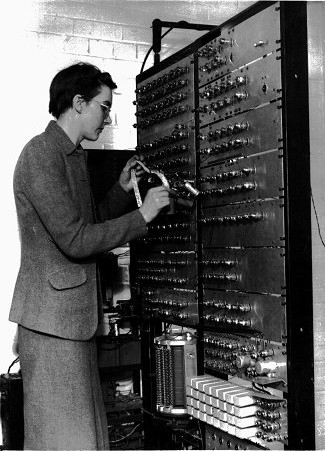
\includegraphics[width=\linewidth]{PLOTS/kathleen-booth.jpg}
\end{columns}
\end{itemize}
\end{frame}

\begin{frame}[fragile]{Programming languages}
\vspace{0.35 cm}
\begin{itemize}\setlength{\itemsep}{0.35 cm}
\item John Mauchly's ``Short Code'' (1949): real mathematical expressions, rather than a series of instructions assigned to registers. However, it had to be typed in a alphanumeric code.

\vspace{0.5 cm}
\begin{minipage}{0.8\linewidth}
\begin{verbatim}
math: X3 =  (  X1 +  Y1 )  /  X1 * Y1
code: X3 03 09 X1 07 Y1 02 04 X1   Y1
\end{verbatim}
\end{minipage}

\vspace{0.5 cm}
\uncover<2->{Intended to make UNIVAC easier for clients to use, but it was interpreted in real time and hence 50$\times$ slower than direct machine code.}
\end{itemize}
\end{frame}

\begin{frame}[fragile]{Programming languages}
\vspace{0.35 cm}
Grace Hopper (Naval Commander and Eckert–Mauchly's first Director of Automatic Programming) wanted computers to understand English words as commands.

\begin{columns}
\column{0.7\linewidth}
\vspace{0.25 cm}
\begin{onlyenv}<1>
\begin{itemize}
\item FLOW-MATIC (1955): compiled, not interpreted

\vspace{0.1 cm}
\tiny
\begin{verbatim}
 (0)  INPUT INVENTORY FILE-A PRICE FILE-B ; OUTPUT PRICED-INV FILE-C
  UNPRICED-INV FILE-D ; HSP D .
 (1)  COMPARE PRODUCT-NO (A) WITH PRODUCT-NO (B) ; IF GREATER GO TO
  OPERATION 10 ; IF EQUAL GO TO OPERATION 5 ; OTHERWISE GO TO OPERATION 2 .
 (2)  TRANSFER A TO D .
 (3)  WRITE-ITEM D .
 (4)  JUMP TO OPERATION 8 .
 (5)  TRANSFER A TO C .
 (6)  MOVE UNIT-PRICE (B) TO UNIT-PRICE (C) .
 (7)  WRITE-ITEM C .
 (8)  READ-ITEM A ; IF END OF DATA GO TO OPERATION 14 .
 (9)  JUMP TO OPERATION 1 .
(10)  READ-ITEM B ; IF END OF DATA GO TO OPERATION 12 .
(11)  JUMP TO OPERATION 1 .
(12)  SET OPERATION 9 TO GO TO OPERATION 2 .
(13)  JUMP TO OPERATION 2 .
(14)  TEST PRODUCT-NO (B) AGAINST ; IF EQUAL GO TO OPERATION 16 ;
  OTHERWISE GO TO OPERATION 15 .
(15)  REWIND B .
(16)  CLOSE-OUT FILES C ; D .
(17)  STOP . (END)
\end{verbatim}
\normalsize
\end{itemize}
\end{onlyenv}\begin{onlyenv}<2>
\begin{itemize}
\item MATH-MATIC (1957): also compiled

\vspace{0.1 cm}
\tiny
\begin{verbatim}
(2)  TYPE-IN ALPHA . 
(2A) READ A B C SERVO 4 STORAGE A IF SENTINEL JUMP TO SENTENCE 8 . 
(3)  READ D F SERVO 5 . 
(4)  VARY Y 1 (0.1) 3 SENTENCE 5 THRU 6 . 
(5)  X1 = (7*103*Y*A*SIN ALPHA)3 / (B POW D+C POW E) . 
(6)  WRITE AND EDIT A Y D E X1 SERVO 6 . 
(7)  JUMP TO SENTENCE 2A . 
(8)  CLOSE-INPUT AND REWIND SENTENCE 3 . 
(9)  CLOSE-OUTPUT SENTENCE 6 . 
(10) READ F G H N SERVO 4 STORAGE A IF SENTINEL JUMP TO SENTENCE 20 . 
(11) EXECUTE SENTENCE 3 . 
(12) X2 = (3 ROOT (E-G)+LOG (D+N)) / (F2.6*EXP H) . 
(13) WRITE EDIT F D F X2 SERVO 6 . 
(16) JUMP TO SENTENCE 10 . 
(20) STOP .
\end{verbatim}
\normalsize
\end{itemize}
\end{onlyenv}\begin{onlyenv}<3>
\begin{itemize}
\item COBOL (1959): maybe you've heard of it?

\vspace{0.1 cm}
\tiny
\begin{verbatim}
      $ SET SOURCEFORMAT"FREE"
IDENTIFICATION DIVISION.
PROGRAM-ID.  Multiplier.

DATA DIVISION.

WORKING-STORAGE SECTION.
01  Num1                                PIC 9  VALUE ZEROS.
01  Num2                                PIC 9  VALUE ZEROS.
01  Result                              PIC 99 VALUE ZEROS.

PROCEDURE DIVISION.
    DISPLAY "Enter first number  (1 digit) : " WITH NO ADVANCING.
    ACCEPT Num1.
    DISPLAY "Enter second number (1 digit) : " WITH NO ADVANCING.
    ACCEPT Num2.
    MULTIPLY Num1 BY Num2 GIVING Result.
    DISPLAY "Result is = ", Result.
    STOP RUN.
\end{verbatim}
\normalsize
\end{itemize}
\end{onlyenv}\begin{onlyenv}<4>
\begin{itemize}
\item Coined the terms ``program,'' ``compile,'' and ``bug.''

\begin{center}
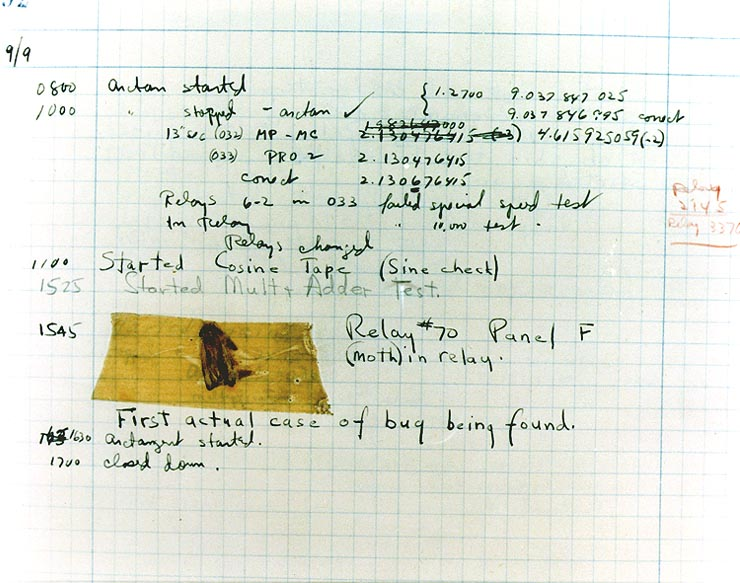
\includegraphics[width=0.7\linewidth]{PLOTS/First_Computer_Bug,_1945.jpg}
\end{center}
\end{itemize}
\end{onlyenv}

\column{0.27\linewidth}
\vspace{0.6 cm}
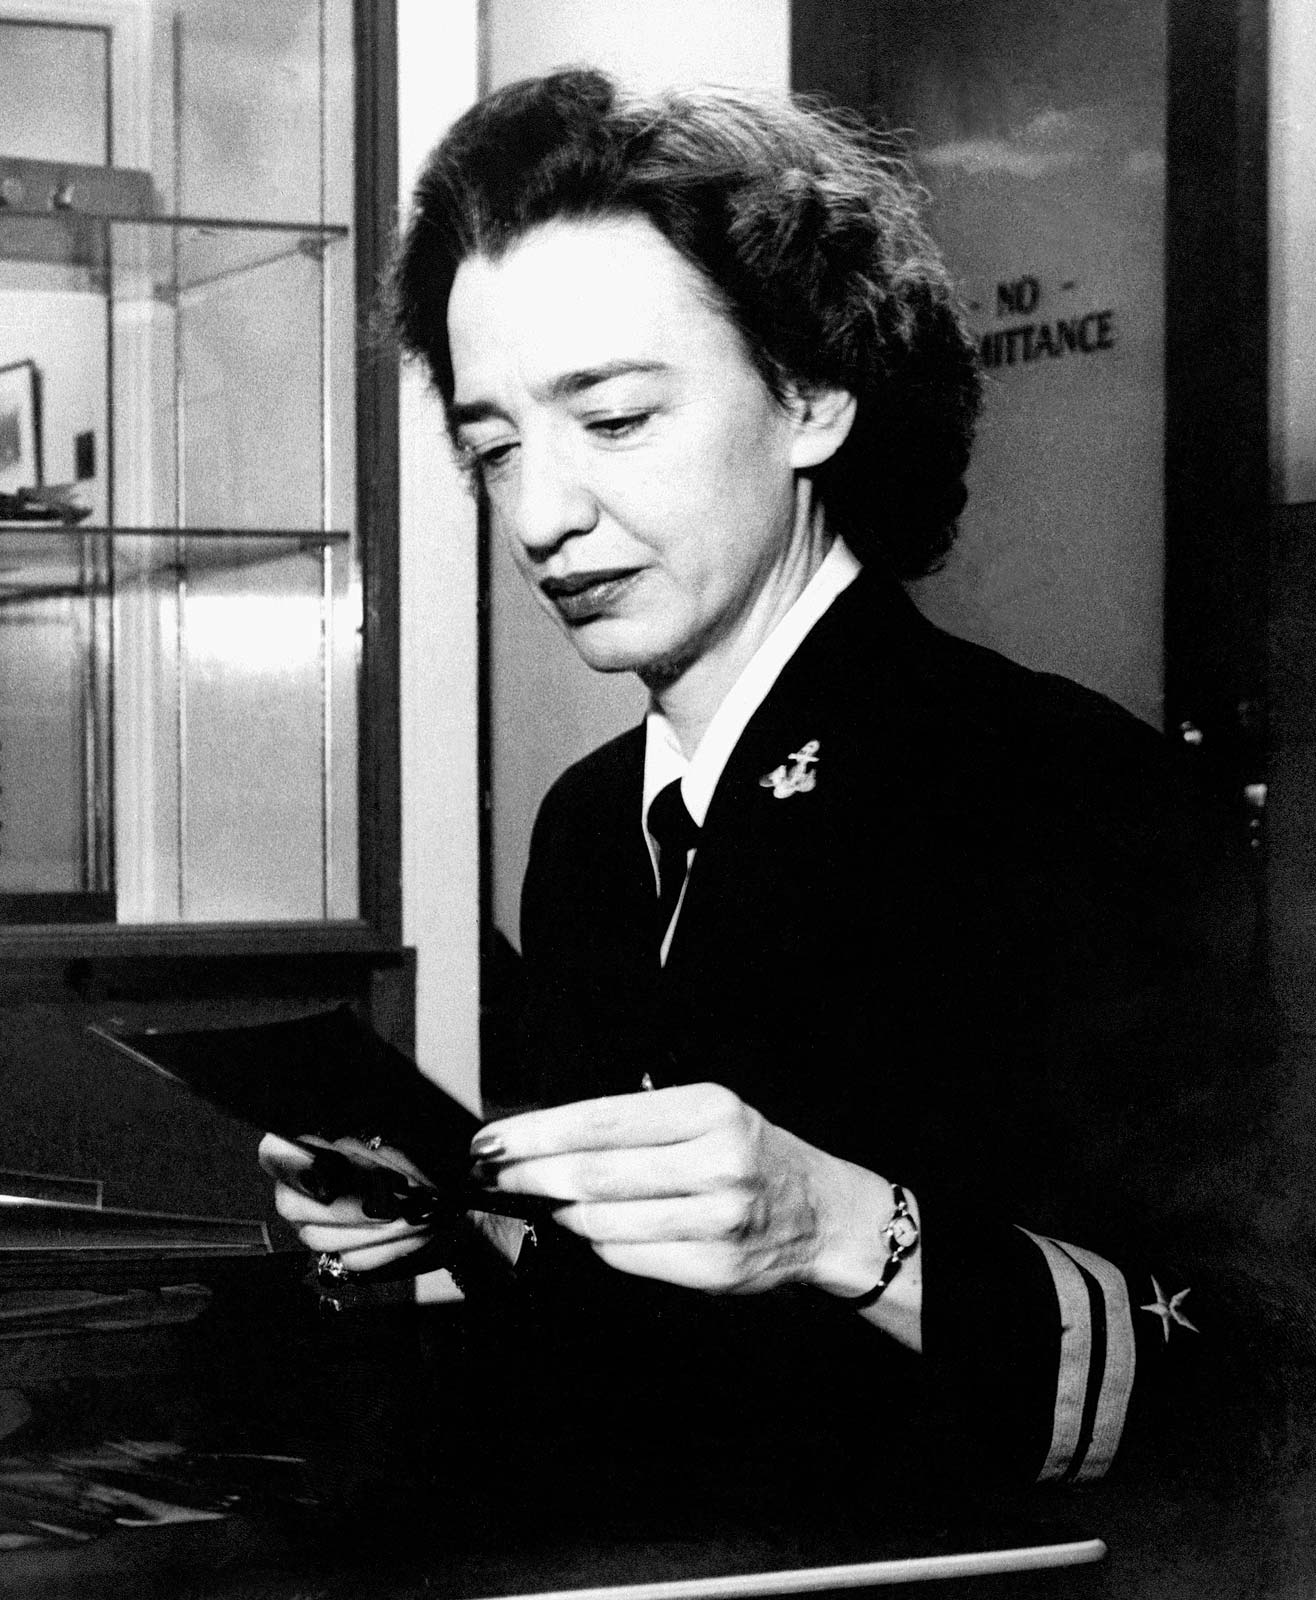
\includegraphics[width=\linewidth]{PLOTS/Grace-Murray-Hopper-Bureau-of-Ordnance-Computation-1946.jpg}
\vspace{0.6 cm}
\end{columns}
\end{frame}

\begin{frame}{Despite UNIVAC's popularity, Eckert–Mauchly Corporation failed}
\vspace{0.165 cm}
\begin{columns}
\column{1.15\linewidth}
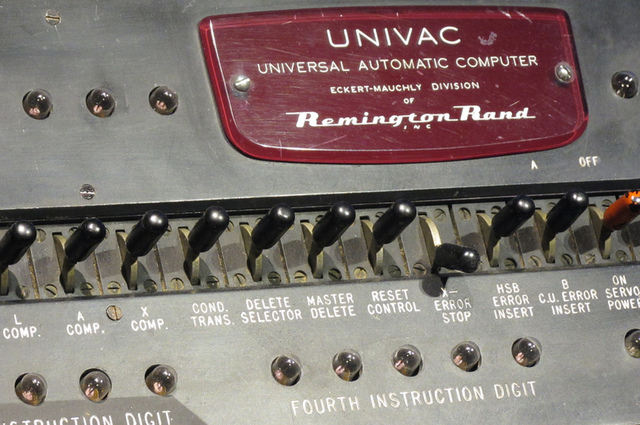
\includegraphics[width=\linewidth]{PLOTS/univac_front_panel.jpg}
\end{columns}
\end{frame}

\begin{frame}[fragile]{A programming language from \raisebox{-0.13 cm}{
\includegraphics[height=0.55 cm]{PLOTS/ibm-logo-1950s}}}
\vspace{0.3 cm}
\begin{itemize}\setlength{\itemsep}{0.35 cm}
\item IBM had been in business since 1911 as Computing-Tabulating-Recording Company, producing tabulators, time-card machines, scales, and punch-cards.

\vspace{0.25 cm}

\uncover<2->{\hfill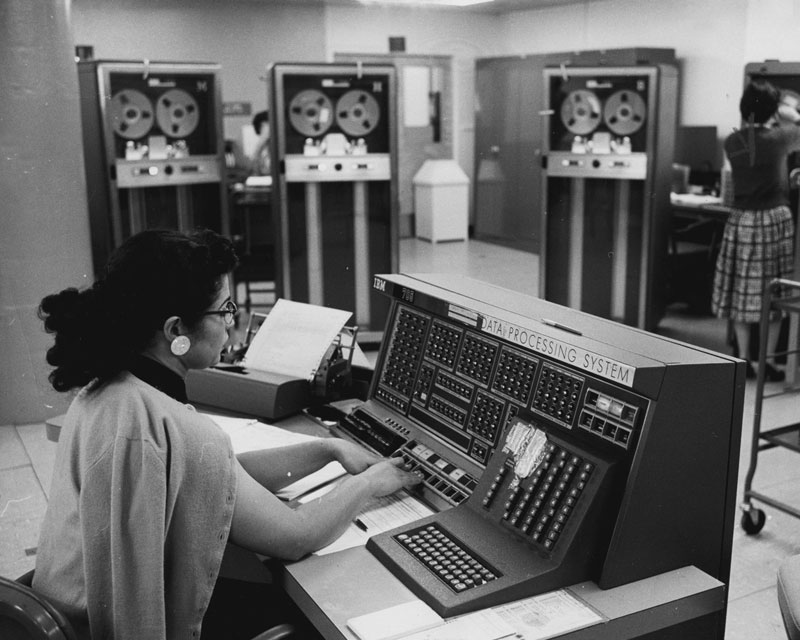
\includegraphics[height=5 cm]{PLOTS/us__en_us__ibm100__700_series__705__800x640.jpg}}

\vspace{-5.25 cm}

\item<2-> After initial reluctance, IBM adopted

the stored-program/tape-drive paradigm.

\item<3-> FORTRAN (John Backus's team, 1956):

\vspace{0.25 cm}
\hspace{-1 cm}\begin{minipage}{0.5\linewidth}
\tiny
\begin{minted}{fortran}
C AREA OF A TRIANGLE - HERONS FORMULA
C INTEGRAL VARIABLES START WITH I,J,K,L,M,N
      READ(5,501) IA,IB,IC
  501 FORMAT(3I5)
      IF(IA.EQ.0 .OR. IB.EQ.0 .OR. IC.EQ.0) STOP 1
      S = (IA + IB + IC) / 2.0
      AREA = SQRT( S * (S - IA) * (S - IB) * (S - IC) )
      WRITE(6,601) IA,IB,IC,AREA
  601 FORMAT(4H A= ,I5,5H  B= ,I5,5H  C= ,I5,8H  AREA= ,F10.2,
     $13H SQUARE UNITS)
      STOP
      END
\end{minted}
\end{minipage}

\vspace{0.25 cm}
\uncover<4->{Compiled, with human-readable words, but unapologetically mathematical and focused on speed. World's first {\it optimizing} compiler.}
\end{itemize}
\end{frame}

\begin{frame}{Other first languages}



\end{frame}



\end{document}

%% Experimental particle physics is an intensely computational field of science. In fact, particle physicists were arguably the first non-secret (non-cryptography) users of digital computers, and have been pushing the boundaries of pattern recognition and throughput ever since. For decades, our unique needs justified custom software at all levels of the stack, maintained "in-house" by physicists, but the situation changed in the 21st century. Machine learning and analysis of web-scale datasets (i.e. "Big Data") has become an industry on its own, under the catch-all name "data science." Physicists are responding by adopting data science toolsets and methodologies, integrating them with traditional physics software, though the process is ongoing and differs in degree across physics groups. 

%% This talk will present a big picture of how experimental particle physicists have used data analysis software in the past 75 years, how our needs have dictated a choice of programming languages and toolkits, and how those choices are changing. We'll see how pattern recognition evolved from semi-automated to algorithmic to machine learning, how programming languages transitioned from Fortran to C++ to include a significant mix of Python, and how software was organized from site-custom solutions to standard packages like CERNLIB and ROOT to also include a mix of data science tools. Finally, these choices are not purely technical: communities form around software tools, and integrating toolsets integrates physicists with the larger world.

% "neural" and (publication_info.cnum:C85-06-25 or publication_info.cnum:C87-02-02.2 or publication_info.cnum:C89-04-10 or publication_info.cnum:C90-04-09 or publication_info.cnum:C91-03-11 or publication_info.cnum:C92-09-21 or publication_info.cnum:C94-04-21 or publication_info.cnum:C95-09-18 or publication_info.cnum:C97-04-07 or publication_info.cnum:C98-08-31 or publication_info.cnum:C00-02-07 or publication_info.cnum:C01-09-03.1 or publication_info.cnum:C03-03-24.1 or publication_info.cnum:C04-09-27 or publication_info.cnum:C06-02-13 or publication_info.cnum:C07-09-02.1 or publication_info.cnum:C09-03-21 or publication_info.cnum:C10-10-18.4 or publication_info.cnum:C12-05-21.3 or publication_info.cnum:C13-10-14.1 or publication_info.cnum:C15-04-13 or publication_info.cnum:C16-10-14 or publication_info.cnum:C18-07-09.6 or publication_info.cnum:C19-11-04 or publication_info.cnum:C21-05-17.1)

% curl -s 'https://inspirehep.net/api/literature?sort=mostrecent&size=25&page=1&q=%28publication_info.cnum%3AC85-06-25%20or%20publication_info.cnum%3AC87-02-02.2%20or%20publication_info.cnum%3AC89-04-10%20or%20publication_info.cnum%3AC90-04-09%20or%20publication_info.cnum%3AC91-03-11%20or%20publication_info.cnum%3AC92-09-21%20or%20publication_info.cnum%3AC94-04-21%20or%20publication_info.cnum%3AC95-09-18%20or%20publication_info.cnum%3AC97-04-07%20or%20publication_info.cnum%3AC98-08-31%20or%20publication_info.cnum%3AC00-02-07%20or%20publication_info.cnum%3AC01-09-03.1%20or%20publication_info.cnum%3AC03-03-24.1%20or%20publication_info.cnum%3AC04-09-27%20or%20publication_info.cnum%3AC06-02-13%20or%20publication_info.cnum%3AC07-09-02.1%20or%20publication_info.cnum%3AC09-03-21%20or%20publication_info.cnum%3AC10-10-18.4%20or%20publication_info.cnum%3AC12-05-21.3%20or%20publication_info.cnum%3AC13-10-14.1%20or%20publication_info.cnum%3AC15-04-13%20or%20publication_info.cnum%3AC16-10-14%20or%20publication_info.cnum%3AC18-07-09.6%20or%20publication_info.cnum%3AC19-11-04%20or%20publication_info.cnum%3AC21-05-17.1%29' 2>&1 > all-chep-papers.json

%% {
%%     "C85-06-25": 1,
%%     "C87-02-02.2": 2,
%%     "C89-04-10": 3,
%%     "C90-04-09": 4,
%%     "C91-03-11": 5,
%%     "C92-09-21": 6,
%%     "C94-04-21": 7,
%%     "C95-09-18": 8,
%%     "C97-04-07": 9,
%%     "C98-08-31": 10,
%%     "C00-02-07": 11,
%%     "C01-09-03.1": 12,
%%     "C03-03-24.1": 13,
%%     "C04-09-27": 14,
%%     "C06-02-13": 15,
%%     "C07-09-02.1": 16,
%%     "C09-03-21": 17,
%%     "C10-10-18.4": 18,
%%     "C12-05-21.3": 19,
%%     "C13-10-14.1": 20,
%%     "C15-04-13": 21,
%%     "C16-10-14": 22,
%%     "C18-07-09.6": 23,
%%     "C19-11-04": 24,
%%     "C21-05-17.1": 25,
%% }

% 2028 HL-LHC LHCb: https://iopscience.iop.org/article/10.1088/1742-6596/706/2/022002
% 20,000-100,000 events per second
% but really just 20,000: https://cds.cern.ch/record/1701361/files/LHCB-TDR-016.pdf

% 2028 HL-LHC ATLAS: https://cds.cern.ch/record/2285584
% 10,000 events per second

% 2028 HL-LHC CMS: https://cds.cern.ch/record/2020886
% 5000 to 7500 events per second

% 2018 ATLAS: https://cds.cern.ch/record/2725146
% 1200 events per second

% 2017 CMS: http://cds.cern.ch/record/2297540
% 1000 events per second

% ATLAS fact sheet: https://cds.cern.ch/record/1457044/files/ATLAS%20fact%20sheet.pdf
% says 1000 million events recorded per year, from 200 events per second (which would be 6000 million/year, but close enough)

% CMS Run I: https://cms.cern/detector/triggering-and-data-acquisition
% says 100 events per second: ~3000 million events per year

% 2012 LHCb: https://inspirehep.net/literature/1211038
% says 3000 events per second: 90,000 million events per year
% LHCb TDR (http://cds.cern.ch/record/630828) says 200 events per second

% 2009 D0 run II: https://inspirehep.net/literature/812698
% 50-100 events per second

% 1988 CDF run I: https://inspirehep.net/literature/262056
% 20-30 events per second

% 1982 UA1: https://inspirehep.net/literature/176681
% says 10 events per second (limited by tape): 300 million per year

%%% Madeleine Isenberg's scanner salary in 1962: $1.75/hour, over the $1/hour minimum wage; would be worth $15.50/hour today.
